\documentclass[12pt]{article}
\pagestyle{empty}
\textheight = 10in
\addtolength{\oddsidemargin}{-.875in}
	\addtolength{\evensidemargin}{-.875in}
	\addtolength{\textwidth}{1.75in}

	\addtolength{\topmargin}{-.875in}
	\addtolength{\textheight}{1.75in}

\usepackage{graphicx}
\usepackage{hyperref}

% Header, put stuff that impacts the whole document here
\NeedsTeXFormat{LaTeX2e}
\title{Software I Project}
\author{Neil Wilcoxson} 


\begin{document}


\maketitle 

\noindent Link to repository: \newline
\url{https://github.com/neilwilcoxson/yahtzy}

\section*{Abstract}

Over the 26 hours that this project took to complete, about 1400 lines of code were written, a UI was designed, and testing was performed.  The use cases set at the beginning of the project were fulfilled.  However, after reaching the end, it has became apparent that it would be possible to have many more iterations of the development process, adding new features and so on.

\section*{Background}
Yahtzy is an extended digital of Hasbro's popular dice game, Yahtzee.  While playing with physical dice and paper scorecards can be fun, this digital version seeks to make gameplay faster and easier.  Furthermore, the autocalculation and hint features help new players learn how to play the game.

\section*{Schedule}
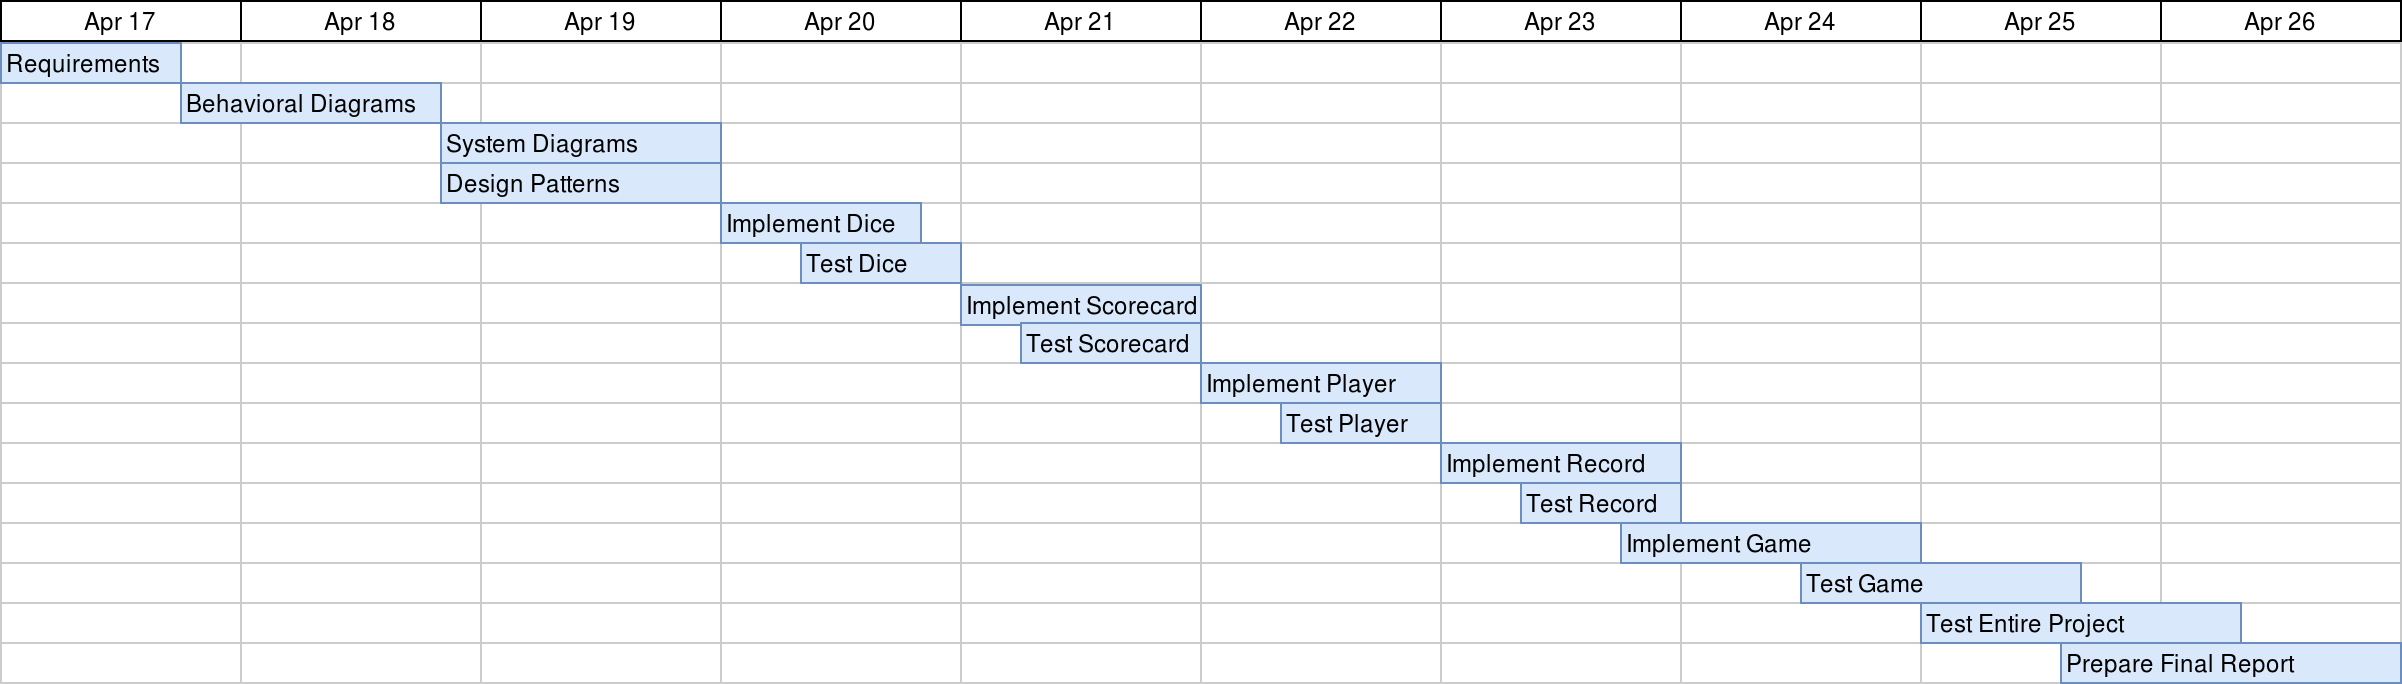
\includegraphics[scale=.21]{diagrams/gnatt.png}

\newpage
\section*{Requirements}
\begin{enumerate}
	\item Player can start a new game
	\item Multiple players can play together
	\item Player can select game options (number of players, name each player, etc.)
	\item Player can roll dice
	\item Player can select which dice to hold
	\item Player can select where to score their rolls
	\item Player can view previous high scores
	\item Player can view their total score
	\item Player can exit the game during gameplay

\end{enumerate}

\section*{Analysis}
\subsection*{Use Cases}
\vspace{.1in}
\hspace{.5in}
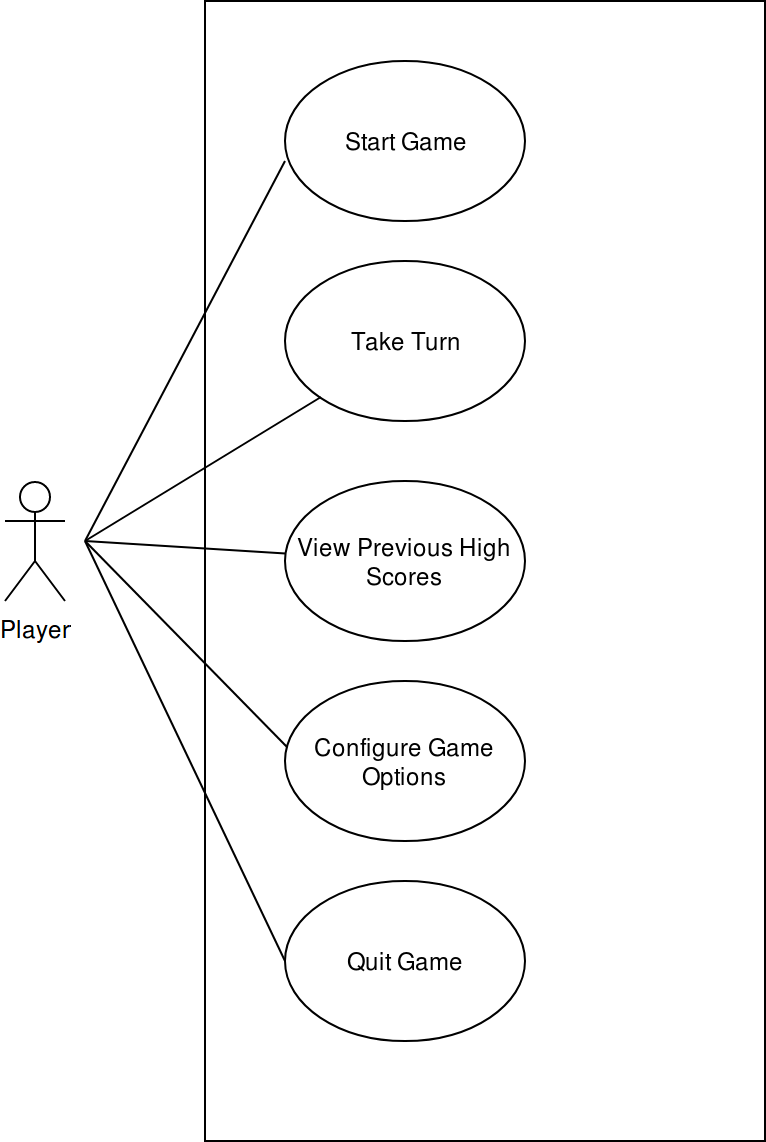
\includegraphics[scale=.3]{diagrams/useCase.png}

\newpage
\begin{list}{}{}

\item {\bf UC1: Starting a game } \newline
{\bf Scope:} Yahtzy Application \newline
{\bf Level:} user goal \newline
{\bf Primary Actor:} Player \newline
{\bf Stakeholders and Interests:} \newline
\indent -Player(s): Want to have fun playing a game \newline
{\bf Precondition(s):} Application is ready to run on the machine \newline
{\bf Postcondition(s):} Game is ready for the player(s) to play \newline \newline
{\bf Main Success Scenario:}
\begin{enumerate}
	\item Player launches the application
	\item Application asks how many players and their names
	\item Application is ready for the first player to take their first turn
\end{enumerate}

\vspace*{.5in}

\item {\bf UC2: Taking a turn} \newline
{\bf Scope:} Yahtzy Application \newline
{\bf Level:} user goal \newline
{\bf Primary Actor:} Player \newline
{\bf Stakeholders and Interests:} \newline
\indent -Player(s): Want to have fun playing a game \newline
\textbf{Precondition(s):} Application is running and game has been started \newline
\textbf{Postcondition(s):} Player’s score is recorded and Application is ready for next player \newline \newline
\textbf{Main Success Scenario:}
\begin{enumerate}
\item Game displays name of player who needs to take their turn
\item Player clicks roll dice
\item Player selects which dice to keep
\item Start again from step 2 up to 2 more times
\item Player selects where to score their roll
\item Control is passed to the next player
\end{enumerate}

\textit{Alternative paths:} \newline
\indent 3.* Player wants to keep all dice they rolled and score immediately \newline
\indent 3.1 Jump to step 5 \newline

\newpage
\item \textbf{UC3: View previous high scores} \newline
\textbf{Scope:} Yahtzy Application \newline
\textbf{Level:} user goal \newline
\textbf{Primary Actor:} Player \newline
\textbf{Stakeholders and Interests:} \newline
\indent -Player(s): Want to have fun playing a game \newline
\textbf{Precondition(s):} Application is running \newline
\textbf{Postcondition(s):} List of high scores is displayed \newline \newline
\textbf{Main Success Scenario:}
\begin{enumerate}
\item Player clicks the high scores button
\item Application displays a list of previous high scores (if any)
\end{enumerate}

\end{list}

\subsection*{Business Rules}
\begin{enumerate}
\item Scores should be calculated by the application rather than by the player.
\item When a score category is selected for which no combination of the dice apply, the recorded score should be zero.
\item Players are not eligible for the bonus if they have already recorded a zero in the Yahtzy space.
\end{enumerate}

\subsection*{System Sequence}
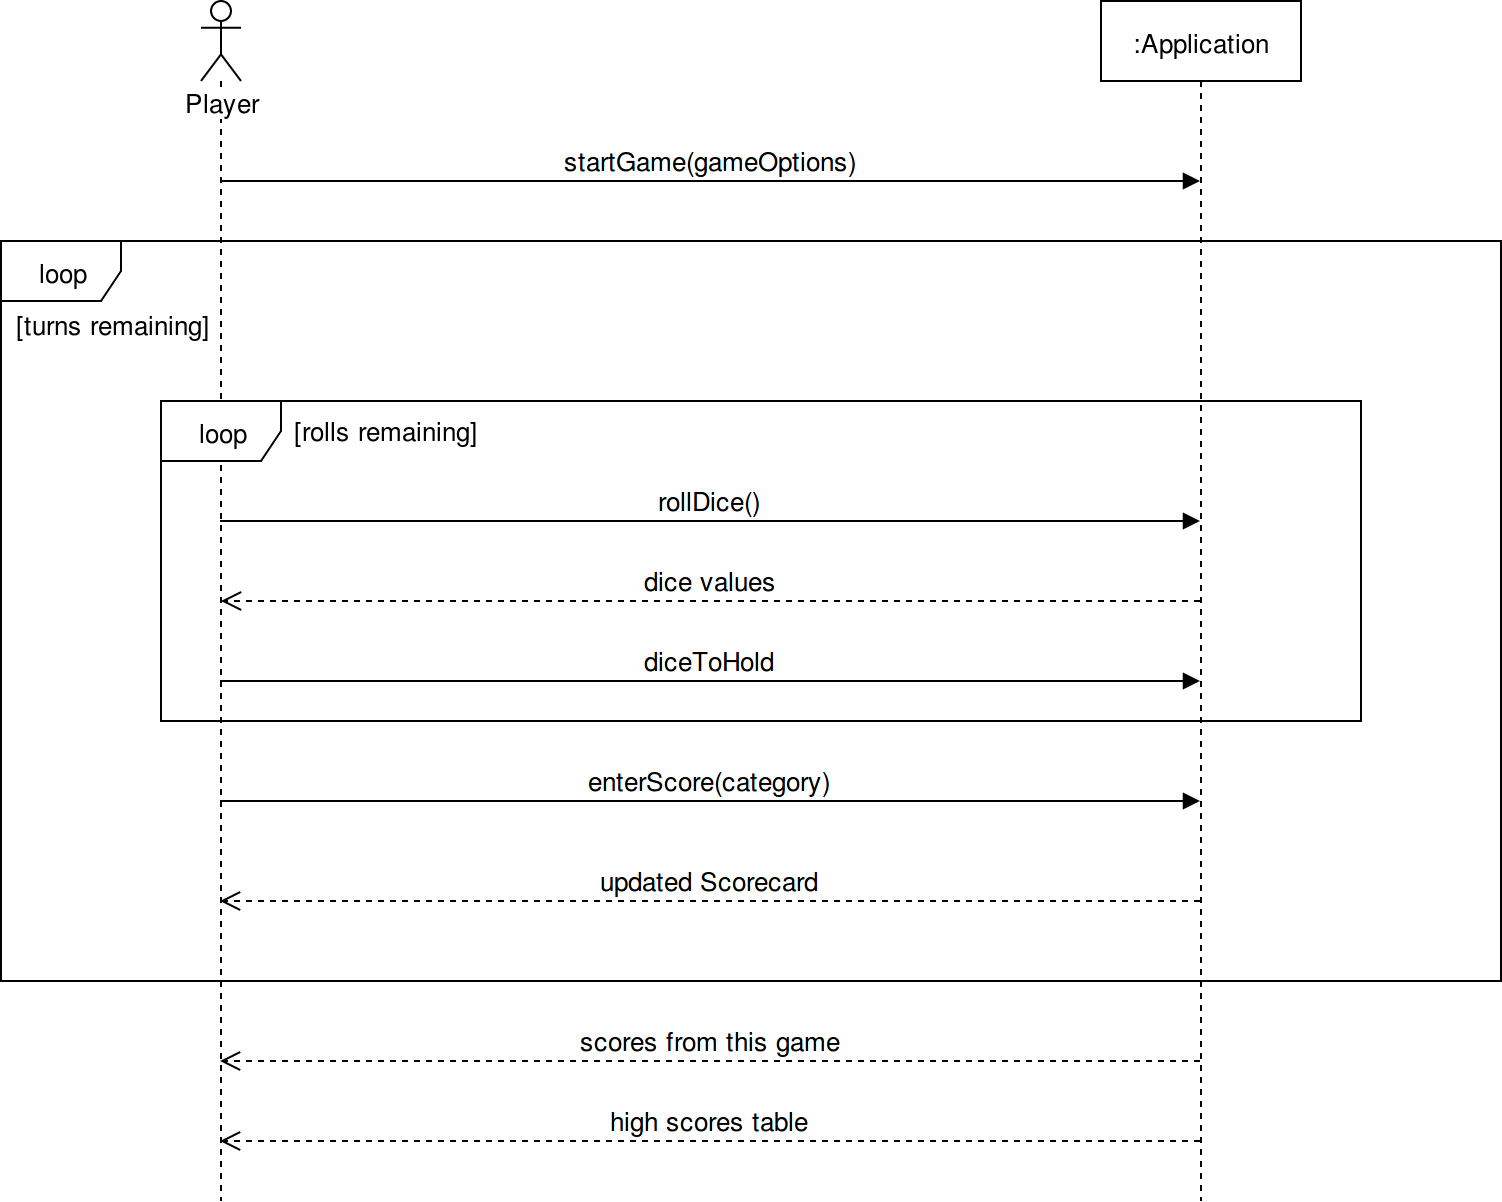
\includegraphics[scale=.28]{diagrams/sequence.png}

\newpage
\subsection*{Operation Contracts}
As stated in Larman's book, not all artifacts will always be needed.  In the case of a game for which nearly everyone is familiar with the rules, these are not necessary in this case.

\section*{Design}
\subsection*{Concepts}
The main conepts were mostly based on the physical objects involved in playing the game (scorecard, dice, player), along with well understood objects like the game and record.  \newline \vspace{.2in}

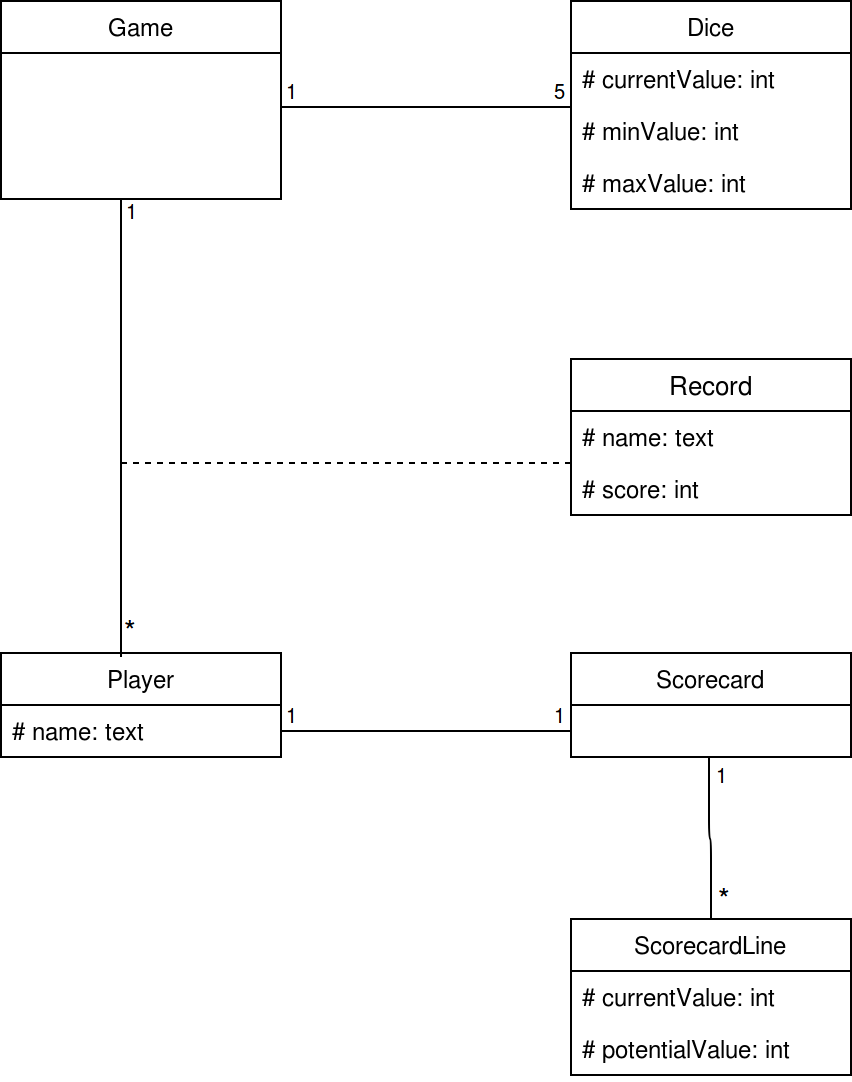
\includegraphics[scale=.38]{diagrams/domainModel.png}

\newpage
\subsection*{GRASP}
\begin{list}{}{}
\item \textbf{Information Expert}\newline
The scorecard is the information expert.  Given several dice, it knows how to score them in each category.

\item \textbf{Creator}\newline
The GUI class creates all ofthe GUI elements.

\item \textbf{Controller}\newline
The Game class controls all aspects of execution of the application.

\item \textbf{Low Coupling}\newline
Simple public methods are created to prevent outside classes from having to call multiple private or protected methods.

\item \textbf{High Cohesion}\newline
Each object is responsible only for doing things directly related to it.  If it is unrelated it is delegated to another class.

\item \textbf{Polymorphism}\newline
Polymorphism is used heavily in the ScorecardLine classes for which each method of scoring has its own class which extends the abstract ScorecardLine class.

\item \textbf{Pure Fabrication}\newline
Some classes do not correspond to a real life object.  For example, MenuHelper is not the menu itself, but it helps perform actions relating to the menu.

\item \textbf{Indirection}\newline
The Game object mediates between the GUI and other game elements.

\item \textbf{Protected Variations}\newline
The main source of variability is user input.  The objects responsible for gathering this information verify the input, and do not pass it along if it is known to be invalid.

\end{list}

\vspace*{.15in}
\subsection*{Design Patterns}
Although many more design patterns were used in the making of this application, here are five major ones.

\begin{enumerate}
\item \textbf{Polymorphism} \newline
All of the scorecard categories inherit from a common ScorecardLine class.  This allows them each to implement their own method for scoring the dice, which is taken advantage of by dynamic binding.
\item \textbf{Facade}\newline
The Game class is a Facade as it arranges all of the game logic for the GUI.  Thus the GUI does not have to interact with each element of game logic directly.

\newpage

\item \textbf{Bridge}\newline
Certain methods of each class are implemented with compatibility in mind.  For example, the Game class implements a getDiceValues method, because the GUI does not need to know about the enitre Dice object, but rather just the values.

\item \textbf{Chain of Responsibility}\newline
Almost every class implements Chain of Responsibility.  When the game wants to score the current dice roll in a particular category, it does not have to contact the ScorecardLine directly.  Instead the game contacts the scorecard.  The scorecard knows what to do, but the game doesn't need to know how it is implemented.
\item \textbf{Observer}\newline
In order to respond to the GUI, the Observer pattern is used.  The buttons present in the GUI are observered and the appropraite repsonse is initiated when the buttons are clicked.
\end{enumerate}

\section*{Implementation}
This application was implemented using Java SE using Swing as the front end.  The source code is available at the repository for the project:\newline
\url{https://github.com/neilwilcoxson/yahtzy}\newline\newline
\noindent The logical line count for the entire application at the time of this report was 1344 lines.

\section*{Evaluation and Testing}
The logical components of the game were tested using JUnit 5 test cases.  However, the graphical components of the game often had no means for testing via JUnit.  These elements were tested manually.  SpotBugs was also used to help identify bugs.  Furthermore prerelease versions of the game were sent to a small group of beta testers who were asked to make suggestions for improvements to the game.  This suggestions were taken into account before the final release.

\section*{Conclusion}
Over the course of this project, many new things were attempted, and the original plans were modified multiple times.  The main takeaway from this project is the discovery of just how ambiguous Software Engineering can be.  Only when an idea becomes code does it become more concrete.  Even then, what the client wanted can suddenly change.  This project has taken 26 hours up to this point, but that does not mean that it is finished.  Yes, the software fulfills the use cases set out earlier in this document, but there are still many improvements that could be made in potential future revisions.  The UI could be more elegant, there could be more gameplay modes, and it could even have networked multiplayer capabilities.  In this sense, no project of this sort is ever really done.

\end{document}






